\section{Problem 1: WARM-UP}\label{problem-1-warm-up}
Original image \cref{fig1} for question \textbf{(a)} \& \textbf{(b)}.
\begin{figure}
    \centering
    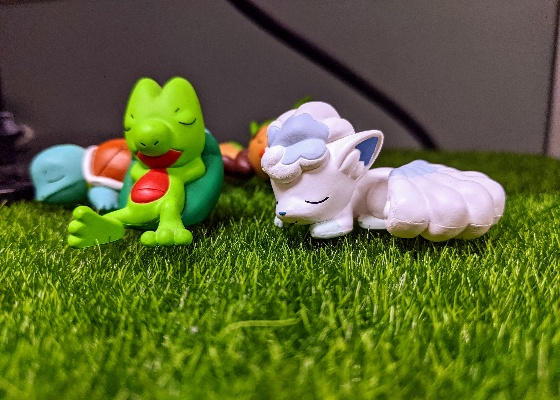
\includegraphics[width=0.7\textwidth]{image/sample1.jpg}
    \caption{\textbf{sample1.jpg}}
    \label{fig1}
\end{figure}

\textbf{(a)} Convert the given color image, \textbf{sample1.jpg}, to a grayscale image named \textbf{1\_result.jpg}.

\textbf{Motivation}
Be familiar with \texttt{Pillow (PIL)} \& \texttt{NumPy}.

\textbf{Approach}
Define \texttt{rgb2gray} function \(\mbox{Grayscale} = 0.2989 * r + 0.5870 * g + 0.1140 * b\) with following \href{https://stackoverflow.com/questions/12201577/how-can-i-convert-an-rgb-image-into-grayscale-in-python}{Stackoverflow reference}.

Note: The coefficient is designed that the human eye is most sensitive to the intensity region. We could also adjust them to get different results.

\textbf{Performance of results}
Result of problem 1(a): \textbf{1\_result.jpg} \cref{fig1a}.
\begin{figure}
    \centering
    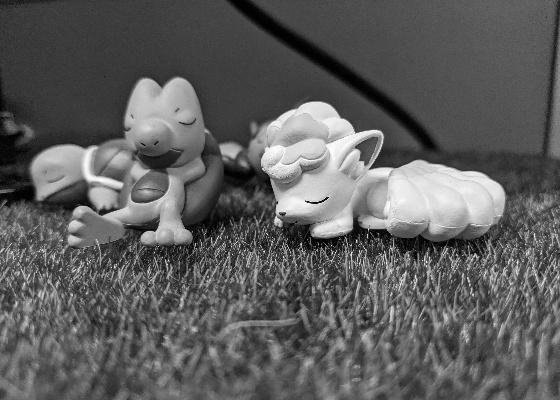
\includegraphics[width=0.7\textwidth]{image/1_result.jpg}
    \caption{\textbf{1\_result.jpg} Colorful to grayscale}
    \label{fig1a}
\end{figure}

\textbf{Discussion}
It looks good. ;-)


\textbf{(b)} Perform horizontal flipping on \textbf{sample1.jpg} and output the result as \textbf{2\_result.jpg}.

\textbf{Motivation}
Be familiar with \texttt{Pillow (PIL)} \& \texttt{NumPy}.

\textbf{Approach} 
Reverse the order of \textbf{column} a.k.a \textbf{second axis} of image array.

\textbf{Performance of results}
Result of problem 1(b): \cref{fig1b}.
\begin{figure}
    \centering
    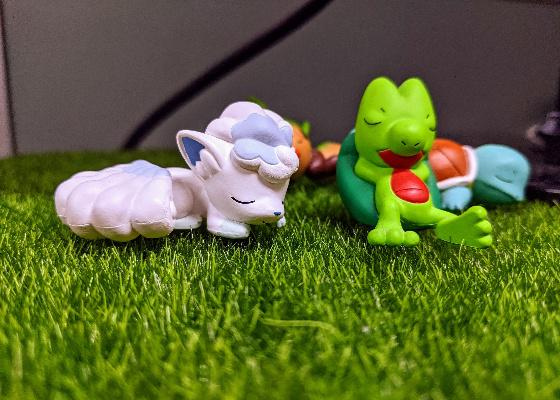
\includegraphics[width=0.7\textwidth]{image/2_result.jpg}
    \caption{\textbf{2\_result.jpg} Horizontal flipping}
    \label{fig1b}
\end{figure}

\textbf{Discussion}
It looks good. ;-)
